%%%%%%%%%%%%%%%%%%%% author.tex %%%%%%%%%%%%%%%%%%%%%%%%%%%%%%%%%%%
%
% sample root file for your "contribution" to a proceedings volume
%
% Use this file as a template for your own input.
%
%%%%%%%%%%%%%%%% Springer %%%%%%%%%%%%%%%%%%%%%%%%%%%%%%%%%%


\documentclass{svproc}
%
% RECOMMENDED %%%%%%%%%%%%%%%%%%%%%%%%%%%%%%%%%%%%%%%%%%%%%%%%%%%
%

% to typeset URLs, URIs, and DOIs
\usepackage{url}
\def\UrlFont{\rmfamily}

\begin{document}
\mainmatter              % start of a contribution
%
\title{Efficient Algebraic Multigrid Preconditioners \\on Clusters of GPUs}
%
%\titlerunning{Hamiltonian Mechanics}  % abbreviated title (for running head)
%                                     also used for the TOC unless
%                                     \toctitle is used
%
\author{Ambra Abdullahi Hassan\inst{1}%
\and Valeria Cardellini\inst{1} \and Pasqua D'Ambra\inst{2} \and \\ 
Daniela di Serafino\inst{3} \and  Salvatore Filippone\inst{4}}
%
%\authorrunning{} % abbreviated author list (for running head)
%
%%%% list of authors for the TOC (use if author list has to be modified)
\tocauthor{Ivar Ekeland, Roger Temam, Jeffrey Dean, David Grove,
Craig Chambers, Kim B. Bruce, and Elisa Bertino}
%
\institute{Universit\`a degli Studi di Roma ``Tor Vergata'', Roma, Italy\\
 \email{\{ambra.abdullahi,cardellini\}@uniroma2.it}
\and
Istituto per le Applicazioni del Calcolo ``Mauro Picone'', CNR, Napoli, Italy\\
 \email{pasqua.dambra@cnr.it}
\and
Universit\`a degli Studi della Campania ``Luigi Vanvitelli'', Caserta, Italy
\email{daniela.diserafino@unicampania.it}
\and
 Cranfield University, Cranfield, UK\\
 \email{salvatore.filippone@cranfield.ac.uk}
}
\maketitle              % typeset the title of the contribution

\begin{abstract}
Many scientific applications require the solution of large and sparse linear systems of equations using iterative methods, this operation accounting for a large percentage of the computing time. In these cases, the choice of the preconditioner is crucial for the convergence of the iterative method.
Given the broad range of applications, great effort has been put in the development of efficient  preconditioners ensuring algorithmic scalability: in this sense, multigrid methods have been proved to be particularly promising.
Additionally, the advent of GPUs, now found in many of the fastest supercomputers, poses the problem of implementing efficiently these algorithms on highly parallel architectures; this is made more difficult by the fact that the solution of sparse triangular systems, a common kernel in many types of preconditioners, is extremely inefficient on GPUs. 

In this paper, we use the PSBLAS and MLD2P4 libraries to explore various issues that affect the efficiency of multilevel preconditioners on GPUs, both in terms of execution speed and exploitation of computational cores, as well as the algorithmic efficiency in guaranteeing convergence to solution in a number of iterations independent of the parallelism degree. 
We investigate these issues 
%are investigated 
in the context of linear systems arising from groundwater modeling application of the filtration of 3D incompressible single-phase flows through %anisotropic 
porous media.

\end{abstract}
%
\section{Introduction}

Many engineering and scientific applications often require the solution of
linear systems
 \begin{equation}
 Ax = b, \qquad x,b \in \Bbb{R}^n,\, A\in \Bbb{R}^{n\times n},
\label{eq:linsys}
\end{equation}
where the matrix $A$ is large and sparse. In our context, \emph{large}
means millions or even billions of unknowns, whereas
\emph{sparse} means that most coefficients in $A$ are zero and it is
convenient to employ special storage formats. In many applications,
and specifically in the test cases discussed in this paper, the matrix
$A$ is also symmetric and positive definite. 

The solution of such systems is achieved by using either direct or iterative methods. 
However, for large and sparse linear systems, direct methods are  difficult to implement in parallel
because of their recursive nature and often suffer from high computational complexity~\cite{Templates}.  
Therefore, a more viable alternative is to use iterative solvers and Krylov
subspace methods are the most widely used class of these solvers~\cite{MR1990645}. 
%The most widely used solvers for systems of this type are Krylov subspace methods~\cite{MR1990645}.
Their time to solution is determined by the number
of iterations performed and by the time per iteration, and hence their 
efficiency is the result of a tradeoff between iteration complexity and speed of convergence. 
A critical feature is the application of preconditioning,
corresponding, e.g., to a transformation of the form
\begin{equation}\label{eq:preclinsys}
M^{-1}Ax=M^{-1}b,
\end{equation} 
which is aimed at speeding up the convergence of Krylov methods through the improvement of
the ``quality'' of the system matrix. Note that the
product $M^{-1}A$ is not computed explicitly, but the Krylov solvers
are modified so that it is obtained by performing at each iteration
the computation of $M^{-1} v$, where $v$ is a suitable vector. 

Multigrid methods are widely used as preconditioners, because they are optimal,
in the sense that their computational cost grows linearly with the number of unknowns
when the linear systems come from the discretization of elliptic partial differential
equations~\cite{Vassilevski2008}.
Many efforts have been performed to extend their efficiency
to more general systems, often the direction of a complete
algebraic approach, where no information on the origin of the problem
is exploited. In this case, they are called Algebraic MultiGrid (AMG) methods~\cite{Stuben2001}.

The linear complexity of AMG preconditioners generally
translates into algorithmic scalability, i.e., the number of iterations
of AMG-preconditioned Krylov solvers does not depend on the size of the
problem. This allows efficient parallel implementations on multiple CPUs,
for example through a domain decomposition approach, in which rows of
the matrix are assigned to different computing nodes.
The diffusion of General Purpose Graphics Processing Units (GPGPUs),
currently found in many of the fastest supercomputers on the Top 500 list
(\url{https://www.top500.org/lists/}), requires the exposition of a high
degree of parallelism, because GPUs are high-throughput many-core processors.
Since AMG methods are obtained by combining different components (smoother,
coarsening algorithm, coarsest-level solver, restriction and prolongation operators),
a full exploitation of GPU capabilities requires each component to be optimized
for this type of architecture.

In this work, we focus on the choice and implementation of AMG smoothers
and coarsest-level solvers capable of harnessing the computational power offered by
a cluster of GPUs. We consider block-Jacobi smoothers and solvers that use sparse
approximate inverses to perform the local solves required by each block, instead of typical
incomplete factorization methods. The choice of sparse approximate inverses
is motivated by the much larger amount of parallelism exposed by
sparse matrix-vector products as compared to the parallelism available
in sparse triangular solves. Furthermore, suitable implementations of sparse approximate
inverse preconditioners have already proved their efficiency on a single GPU (see, e.g.,
\cite{BERTACCINI2016693,Lukash:2012}). 
In our work, the smoothers and local solvers are used within
the AMG framework offered by the MLD2P4 package of preconditioners~\cite{mld-toms} 
and exploiting sparse matrix data structures and Krylov solvers from
the PSBLAS  library~\cite{PSBLAS3}. 
We conducted an extensive set of weak scalability tests on the JURECA supercomputer at the J\"ulich Supercomputing Centre (JSC), 
using a groundwater modelling application developed at JSC. 
To quantify the gain in efficiency and performance using the cluster of GPUs, we also ran tests only on CPUs. 
Our results show scalability up to 128 GPUs and 256 millions equations.

%and are analyzed in terms of both execution speed and algorithmic scalability.
To the best of our knowledge, the selected AMG smoothers and local solvers have not been
considered in other AMG preconditioners tailored for GPUs~\cite{BellDaltonOlson:2012, }. 

%\textbf{Aggiungere biblio:
%Bell, Dalton, Olson; Park, Smelianskiy, Yang, ...; Rupp, Weinbub}. 

Furthermore, most results have been so far presented on a single GPU; 
for example, Richter et al.~\cite{Richter:2014} presented the implementation for discrete elliptic field problems 
using the CUSP library. 

In this work, we do not consider the setup phase of the preconditioner,
which will be the subject of future work. 
Of course, an efficient AMG setup on multiple GPUs is important for the overall efficiency of the
preconditioner. Nevertheless, in situations where we need to solve multiple
linear systems with the same coefficient matrix, it is desirable to obtain
the best possible efficiency during the solution phase even at the expense of a
longer setup time, because this will be amortized over multiple
solution steps.

The remainder of this article is organized as follows. In Section~\ref{AMG} we briefly describe AMG preconditioners,
identifying their main sparse matrix kernels. In Section~\ref{SLA-GPU}, we discuss the main issues
concerning the implementation of these kernels on GPUs. In Section~\ref{results} we illustrate the
behaviour of the AMG preconditioners on a cluster of GPUs on linear systems coming from a
a groundwater modelling applications. 
We conclude in Section~\ref{sec:concl} with some final remarks.  
%

\section{Algebraic Multigrid Preconditioners\label{AMG}}
%
%MultiGrid methods are widely used as preconditioners of iterative
%Krylov solver for sparse linear systems. 
%They are very efficient methods, having linear computational
%complexity and hence perfect scalability, when 
%sparse and large linear systems stemming
%from the discretization of some scalar elliptic Partial Differential
%Equations (PDEs) have to be solved~\cite{Vassilevski2008}. 
%Many efforts are related to extend their efficient applicability also
%to more general systems, in particular in the direction of a complete
%algebraic approach, where no information on a possible geometric
%origin of the problem is exploited. In this last case, they are called
%Algebraic MultiGrid (AMG) or Algebraic Multilevel
%methods~\cite{Stuben2001}. 
Multigrid methods achieve  their efficiency by the recursive application
of two complementary processes: \emph{relaxation} and \emph{coarse-grid
correction}.
%
\begin{figure}[t]
\begin{center}
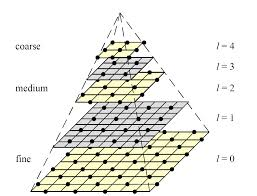
\includegraphics[width=.75\textwidth]{multilevel.png}
\caption{A MultiGrid hierarchy.\label{hierarchy}}
\end{center}
\end{figure}
%
Relaxation consists in the application of an iterative method, such as
Jacobi or Gauss-Seidel, to reduce highly oscillatory error components,
while the coarse-grid correction corresponds to the solution of the
resulting residual equation in an appropriately chosen coarse space,
aimed at reducing the leftover error components. The recursive application
of this procedure leads to a \emph{multilevel hierarchy} of spaces,
depicted in Fig.~\ref{hierarchy}. 

In the classical multigrid approach, the coarser grid and the interpolation
operator for transferring the coarse-grid solution to the original (fine) grid are
predefined by the geometry of the problem. Conversely,
AMG methods address the setup phase, known as~\emph{coarsening process},
in an automatic way, without using explicit knowledge of the
problem which the linear system originates from, and relying only on the entries of
the system matrix. Here we consider
an algebraic coarsening process based on the aggregation strategy,
where coarse-grid unknowns are aggregates of original
unknowns. In particular, the AMG preconditioners available in the MLD2P4
library~\cite{mld-toms} rely
on a decoupled version of \emph{the smoothed aggregation} algorithm
described in~\cite{BrezinaVanek96,BrezinaVanek99}. This procedure is
currently implemented on the host CPUs; for the sake of space,
we refer the reader to~\cite{mld2p4-2-guide} for details on the related
algorithm and its parallel implementation.

Our aim here is to identify the main linear algebra
operations needed for the application of the AMG preconditioner with
a Krylov solver, since the efficient implementation of these operations on
GPUs is the main focus of this work. 

The application phase of an AMG preconditioner is also known as
multigrid cycle. The most widely used one is the so called symmetric
V-cycle, described in Fig.~\ref{Vcycle}, where the AMG hierarchies of
$nlev$ prolongator operators $P^k$ and of corresponding coarse
matrices, obtained by the standard variational approach
$A^{k+1}=(P^{k+1})^TA^kP^{k+1}$, have been built in the setup phase.
%
\begin{figure}[t]
\begin{center}
\framebox{
\begin{minipage}{.85\textwidth}
\begin{tabbing}
\quad \=\quad \=\quad \=\quad \\[-3mm]
procedure V-cycle$\left(k,A^k,b^k,x^k\right)$ \\[2mm]
\>if $\left(k \ne nlev \right)$ then \\[1mm]
\>\> $x^k = x^k + (M^k)^{-1} \left(b^k - A^k x^k\right)$ \\[1mm]
\>\> $b^{k+1} = (P^{k+1})^T\left(b^k - A^k x^k\right)$ \\[1mm]
\>\> $x^{k+1} =$ V-cycle$\left(k+1,A^{k+1},b^{k+1},0\right)$ \\[1mm]
\>\> $x^k = x^k + P^{k+1} x^{k+1}$ \\[1mm]
\>\> $x^k = x^k + (M^k)^{-T} \left(b^k - A^k x^k\right)$ \\[1mm]
\>else \\[1mm]
\>\> $x^k = \left(A^k\right)^{-1} b^k$\\[1mm]
\>endif \\[1mm]
\>return $x^k$ \\[1mm]
end
\end{tabbing}
\end{minipage}
}
\caption{V-cycle preconditioner.\label{Vcycle}}
\end{center}
\end{figure}
%
$M^k$ represents the matrix
operator corresponding to the basic iterative method applied as smoother
at level $k$. 

The main computational kernels in the application of the preconditioner
are the sparse matrix-vector multiplication and the inversion of  $M^k$.
In the simple case of Jacobi method, $M^k=diag(A^k)$ and hence
inverting $M^k$ corresponds to a highly parallel vector
update operation. On the other hand, more robust iterative methods,
such as the Gauss-Seidel method or incomplete factorizations, are
often required to improve the convergence of the preconditioned solver
applied to general linear systems. In these cases, the inversion of
the corresponding matrix operators requires the solution of triangular
systems, which is a sequential kernel. Therefore, an
efficient parallel implementation of the V-cycle is
strictly related to the availability of iterative
methods which can be formulated in terms of sparse matrix-vector multiplication (SpMV)
and, possibly, vector updates, and to an efficient implementation of the sparse
matrix-vector multiplication.


%
\input{3-gpu_linalg.tex}
% \section{Sparse linear algebra on GPUs}
% Sparse linear algebra on GPU e limitazioni del nucleo risoluzione di sistemi triangolari, uso delle inverse approssimate e focus sulla INVK di PSBLAS.
\section{Results}
Distribuzione dati fatta tenendo conto della geometria (3D) del problema e giustificandola rispetto al vantaggio che fornisce in termini di rapporto calcolo/comunicazione
\paragraph{Aacknowledgement}


%
% ---- Bibliography ----
%
\begin{thebibliography}{6}
%

\bibitem {}


\end{thebibliography}
\end{document}
